\section{DNS and P2P}
\subsection{DNS}
\subsection{Structure of a DNS Message}
\begin{Verbatim}[commandchars=\\\{\}]
    \textcolor{blue}{+---------------------+}
    \textcolor{blue}{|        Header       |}
    \textcolor{blue}{+---------------------+}
    \textcolor{blue}{|       Question      | the question for the name server}
    \textcolor{blue}{+---------------------+}
    \textcolor{blue}{|        Answer       | RRs answering the question}
    \textcolor{blue}{+---------------------+}
    \textcolor{blue}{|      Authority      | RRs pointing toward an authority}
    \textcolor{blue}{+---------------------+}
    \textcolor{blue}{|      Additional     | RRs holding additional information}
    \textcolor{blue}{+---------------------+}
\end{Verbatim}
\begin{itemize}[nosep]
    \item Same format for queries and replies
          \begin{itemize}[nosep]
              \item Query has 0 RRs in Answer/Authority/Additional
              \item Reply includes question, plus has RRs
          \end{itemize}
    \item Authority allows for delegation
    \item Additional for glue, other RRs client might need
\end{itemize}
\subsection{Header Format}
\begin{Verbatim}[commandchars=\\\{\}]
    \textcolor{blue}{                                1  1  1  1  1  1}
    \textcolor{blue}{  0  1  2  3  4  5  6  7  8  9  0  1  2  3  4  5}
    \textcolor{blue}{+--+--+--+--+--+--+--+--+--+--+--+--+--+--+--+--+}
    \textcolor{blue}{|                      ID                       |}
    \textcolor{blue}{+--+--+--+--+--+--+--+--+--+--+--+--+--+--+--+--+}
    \textcolor{blue}{|QR|   Opcode  |AA|TC|RD|RA|   Z    |   RCODE   |}
    \textcolor{blue}{+--+--+--+--+--+--+--+--+--+--+--+--+--+--+--+--+}
    \textcolor{blue}{|                    QDCOUNT                    |}
    \textcolor{blue}{+--+--+--+--+--+--+--+--+--+--+--+--+--+--+--+--+}
    \textcolor{blue}{|                    ANCOUNT                    |}
    \textcolor{blue}{+--+--+--+--+--+--+--+--+--+--+--+--+--+--+--+--+}
    \textcolor{blue}{|                    NSCOUNT                    |}
    \textcolor{blue}{+--+--+--+--+--+--+--+--+--+--+--+--+--+--+--+--+}
    \textcolor{blue}{|                    ARCOUNT                    |}
    \textcolor{blue}{+--+--+--+--+--+--+--+--+--+--+--+--+--+--+--+--+}
\end{Verbatim}
\begin{itemize}[nosep]
    \item ID: match response to query; QR: 0 query/1 response
    \item RCODE: error code
    \item AA: authoritative answer, TC: truncated
    \item RD: recursion desired, RA: recursion available
\end{itemize}
\subsection{Other RR Types}
\begin{itemize}[nosep]
    \item CNAME (canonical name): specifies an alias
          \begin{minted}{html}
        www.google.com.      446199 in CNAME    www.l.google.com
        www.l.google.com.  300 IN  A    72.14.204.147
    \end{minted}
    \item MX record: specifies servers to handle mail for a domain (the part after the @ in email address)
    \item SOA (start of authority)
          \begin{itemize}[nosep]
              \item Information about a DNS zone and the server responsible for the zone
          \end{itemize}
    \item PTR (reverse lookup)

          \verb|18.240.7.129.in-addr.arpa. 3600 IN PTR bayou.cs.uh.edu.|

          \url{https://en.wikipedia.org/wiki/List_of_DNS_record_types}
\end{itemize}

\subsection{Inserting a Record in DNS}
\begin{itemize}[nosep]
    \item Your new startup httpserver.com
    \item Get a block of addresses from ISP
          \begin{itemize}[nosep]
              \item say 212.44.9.128/25
          \end{itemize}
    \item Register helpme.com at GoDaddy.com (for example)
          \begin{itemize}[nosep]
              \item Provide name and address of your authoritative name server (primary and secondary)
              \item Registrar inserts RR pair into the com TLD server:
                    \begin{itemize}[nosep]
                        \item helpme.com NS dns1.httpserver.com
                        \item dns1.helpme.com A 212.44.9.129
                    \end{itemize}
          \end{itemize}
    \item Configure your authoritative server (dns1.helpme.com)
          \begin{itemize}[nosep]
              \item Tyep A record for www.httpserver.com
              \item Type MX record for httpserver.com
          \end{itemize}
    \item Need to provide reverse PTR bindings
          \begin{itemize}[nosep]
              \item e.g. 212.44.9.129 $\rightarrow$ dns1.httpserver.com
          \end{itemize}
    \item Normally, these would go into 9.44.212.in-addr.arpa zone
    \item Problem: you can't run the name server for that domain. Why not?
          \begin{itemize}[nosep]
              \item Your block is 212.44.9.128/25, not 212.44.9.0/24
              \item Whoever has 212.44.9.0/24 would not be happy with you setting their PTR records
          \end{itemize}
    \item Solution: [RFC2317, Classless Delegation]
          \begin{itemize}[nosep]
              \item Install CNAME records in parent zone, e.g. \textcolor{blue}{129.9.44.212.in-­‐addr.arpa CNAME 129.ptr.httpserver.com}
          \end{itemize}
\end{itemize}
\subsection{DNS Security}
\begin{itemize}[nosep]
    \item You go to Starbucks,  how does your browser find www.google.com?
          \begin{itemize}[nosep]
              \item ask local name server, obtained from DHCP
              \item you implicitly trust this server
              \item can return any answer for google.com, including a malicious IP that poses as a man in the middle
          \end{itemize}
    \item How can you know you are getting correct data?
          \begin{itemize}[nosep]
              \item today, you can't
              \item HTTPS can help
              \item DNSSEC extension will allow you to verify
          \end{itemize}
\end{itemize}
\subsection{Cache Poisoning}
\begin{itemize}[nosep]
    \item Suppose you can tronl evil.com. You receive a query for www.evil.com and reply
          \begin{Verbatim}[commandchars=\\\{\}]
              ;; QUESTION SECTION:
              ;www.evil.com.                  IN     A

              ;; ANSWER SECTION:
              www.evil.com.           300     IN     A     212.44.9.144

              ;; AUTHORITY SECTION:
              evil.com.               600     IN     NS    dns1.evil.com.
              evil.com.               600     IN     NS    \textcolor{red}{google.com}.

              ;; ADDITIONAL SECTION:
              \textcolor{red}{google.com.               5     IN     A    212.44.9.155}
          \end{Verbatim}
    \item Glue record pointing to your IP, not Google's
    \item Gets cached!
    \item But how do you get a vimctim to look up evil.com?
    \item You might connect to their mail server and send
          \begin{itemize}[nosep]
              \item HELO www.evil.com
              \item Which their mail server then looks up to see if it corresponds to your IP address (SPAM filtering)
          \end{itemize}
    \item Mitigation (bailiwick checking)
          \begin{itemize}[nosep]
              \item Only accepts glue records from the domain you asked for
          \end{itemize}
    \item Bad guy at Starbucks can sniff or \emph{guess} the ID field the local server will use
          \begin{itemize}[nosep]
              \item Not hard if DNS server generates ID numbers sequentially
              \item Can be done if you force the DNS server to look up something in \emph{your} name server
              \item Guess has 1 in 65535 chance (or does it?)
          \end{itemize}
    \item Now:
          \begin{itemize}[nosep]
              \item Ask the local server to lookup google.com
              \item Spoof the response from google.com using the correct ID
              \item Bogus response arrives before legit one (maybe)
          \end{itemize}
    \item Local server caches first response it receives
          \begin{itemize}[nosep]
              \item Attacker can set a long TTL
          \end{itemize}
\end{itemize}
\subsection{Guessing Query ID}
\begin{figure}[H]
    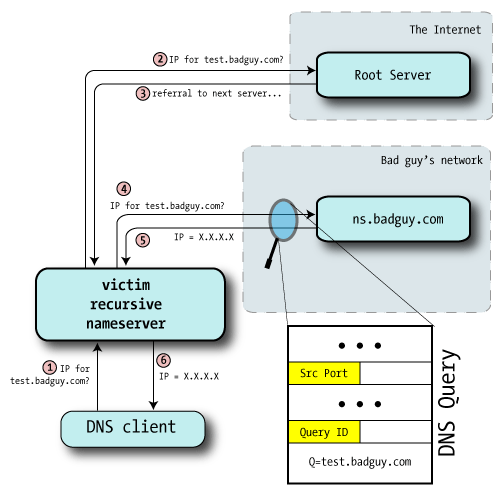
\includegraphics[scale=0.5]{lazy/guessing-query-id.png}
\end{figure}
\url{http://www.unixwiz.net/techtips/iguide-kaminsky-dns-vuln.html}
\subsection{Cache Poisoning}
\begin{figure}[H]
    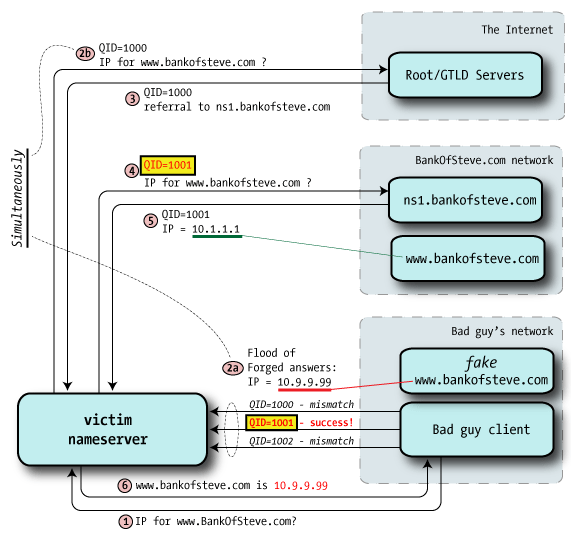
\includegraphics[scale=0.5]{lazy/cache-poisoning.png}
\end{figure}
\url{http://www.unixwiz.net/techtips/iguide-kaminsky-dns-vuln.html}
\subsection{Hijacking Authority Record}
\begin{figure}[H]
    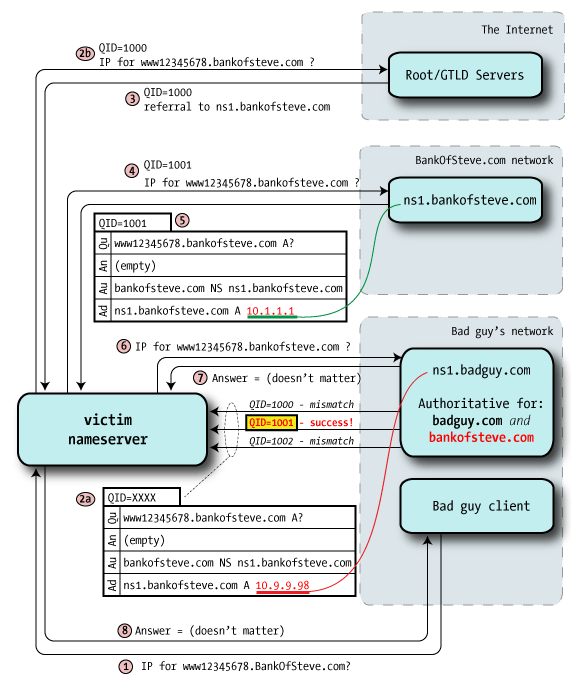
\includegraphics[scale=0.5]{lazy/hijacking.png}
\end{figure}
\url{http://www.unixwiz.net/techtips/iguide-kaminsky-dns-vuln.html}
\subsection{Kaminsky Exploit}
\begin{itemize}[nosep]
    \item If good guy wins the race, you have to wait until the TTL to race again
    \item But\dots
          \begin{itemize}[nosep]
              \item What if you start a new race for AAAA.google.com, AAAB.google.com, \dots?
              \item Forge CNAME responses for each
              \item Circumvents bailiwick checking
          \end{itemize}
\end{itemize}
\subsection{Countermeasures}
\begin{itemize}[nosep]
    \item Randomize ID
          \begin{itemize}[nosep]
              \item Used to be sequential
          \end{itemize}
    \item Randomize source port number
          \begin{itemize}[nosep]
              \item Used to be the same for all requests from the server
          \end{itemize}
    \item Offers some protection, but attack still possible
\end{itemize}
\subsection{Load Balancing using DNS}
\begin{itemize}[nosep]
    \item Return multiple IP addresses (``A'' records) for a name
    \item Benefits
          \begin{itemize}[nosep]
              \item Spread the load evenly across the IP addresses
          \end{itemize}
    \item Problems
          \begin{itemize}[nosep]
              \item Caching, no standard on which address to use, \dots
          \end{itemize}
    \item How to solve these problems?
          \begin{itemize}[nosep]
              \item Poll load to compute return list
              \item \url{https://en.wikipedia.org/wiki/Round-robin_DNS}
          \end{itemize}
\end{itemize}
\subsection{Peer-to-Peer}
\subsection{Client-Server Bottlenecks}
\begin{itemize}[nosep]
    \item Download time can scale linearly ($\bigO{n}$ with $n$ clients)
    \item Scaling up server bandwidth can be expensive
    \item Too expensive to provision for flash crowds
\end{itemize}
\subsection{Peer-to-Peer Systems}
\begin{itemize}
    \item How did it start?
          \begin{itemize}[nosep]
              \item A killer application: file distribution
              \item Free music over the internet (not exactly legal\dots)
          \end{itemize}
    \item Key idea: share storage, content, and bandwidth of individual users
          \begin{itemize}[nosep]
              \item Lots of them
          \end{itemize}
    \item Big challenge: coordinate all of these users
          \begin{itemize}[nosep]
              \item In a scalable way (not $n\times n=n^2$)
              \item With changing population (aka \emph{churn})
              \item With no central administration
              \item With no trust
              \item With large heterogeneity (content, storage, bandwidth, \dots)
          \end{itemize}
\end{itemize}
\subsection{3 Key Requirements}
\begin{itemize}[nosep]
    \item P2P Systems do Three things:
          \begin{enumerate}[nosep]
              \item Help users \emph{determine what they want}
                    \begin{itemize}[nosep]
                        \item Some form of search
                        \item P2P version of Google
                    \end{itemize}
              \item \emph{Locate} that content
                    \begin{itemize}[nosep]
                        \item Which node(s) hold the content?
                        \item P2P version of DNS (map name to location)
                    \end{itemize}
              \item \emph{Download} the content
                    \begin{itemize}[nosep]
                        \item Should be efficient
                        \item P2P form of Akamai
                    \end{itemize}
          \end{enumerate}
\end{itemize}
\subsection{Napster}
\begin{itemize}[nosep]
    \item Search \& Location: central server
    \item Download: contact a peer, transfer directly
    \item Advantages:
          \begin{itemize}[nosep]
              \item Simple, advanced search possible
          \end{itemize}
    \item Disadvantages:
          \begin{itemize}[nosep]
              \item Single point of failure (technical and \dots legal!)
              \item The latter is what got Napster killed
          \end{itemize}
\end{itemize}
\subsection{Gnutella: Flooding on Overlays (2000)}
\begin{itemize}[nosep]
    \item Search \& Location: flooding (with TTL)
    \item Download: direct
\end{itemize}
\subsection{BitTorrent}
\begin{itemize}[nosep]
    \item One big problem with previous approaches
          \begin{itemize}[nosep]
              \item Asymmetric bandwidth
          \end{itemize}
    \item BitTorrent
          \begin{itemize}[nosep]
              \item Search: independent search engines (e.g. PirateBay, isoHunt)
                    \begin{itemize}[nosep]
                        \item Maps keywords $\to$ .torrent file
                    \end{itemize}
              \item Location: centralized \emph{tracker} node per file
              \item Download: chunked
                    \begin{itemize}[nosep]
                        \item File split into many pieces
                        \item Can download from many peers
                    \end{itemize}
          \end{itemize}
    \item How does it work?
          \begin{itemize}[nosep]
              \item Split files into large pieces (245KB - 1MB)
              \item Split pieces into subpieces
              \item Get peers from tracker, exchange info on pieces
          \end{itemize}
    \item Three phases in download
          \begin{itemize}[nosep]
              \item Start: get a piece as soon as possible (random)
              \item Middle: spread pieces fast (rarest piece)
              \item End: don't get stuck (parallel downloads of last pieces)
          \end{itemize}
\end{itemize}
\subsection{BitTorrent Tracker Files}
\begin{itemize}[nosep]
    \item Torrent file (.torrent) describes files to download
          \begin{itemize}[nosep]
              \item Names tracker, server tracking who is participating
              \item File length, piece length, SHA1 hash of pieces
              \item Additional metadata
          \end{itemize}
    \item Client contacts tracker, starts communicating with peers
          \begin{verbatim}
        d8:announce39:http://torrent.ubuntu.com:6969/announce13:announce-
        listll39:http://torrent.ubuntu.com:6969/announceel44:http://
        ipv6.torrent.ubuntu.com:6969/announceee7:comment29:Ubuntu CD
        releases.ubuntu.com13:creation
        datei1272557944e4:infod6:lengthi733837312e4:name29:ubuntu-10.04-
        netbook-i386.iso12:piece lengthi524288e6:pieces28000:…
    \end{verbatim}
          Example tracker from ubuntu.com
    \item Self-scaling: incentivize sharing
          \begin{itemize}[nosep]
              \item If people upload as much as they download, system scales with number of users (no free-loading)
          \end{itemize}
    \item Uses tit-for-tat: only upload to those who give you data
          \begin{itemize}[nosep]
              \item \emph{Choke} most of your peers (don't upload to them)
              \item Order peers by download rate, choke all but $P$ best
              \item Occasionally unchoke a random peer (might become a nice uploader)
          \end{itemize}
\end{itemize}
\subsection{Skype}
\begin{itemize}[nosep]
    \item Real-time communication
    \item Two major challenges:
          \begin{itemize}[nosep]
              \item Finding what host a user is on
              \item Being able to communicate with those hosts
          \end{itemize}
    \item Uses Superpeers for registering presence, searching for where you are
          \begin{itemize}[nosep]
              \item Need bootstrap super-peers
          \end{itemize}
    \item Those Superpeers organize index of users
    \item Making a call
          \begin{itemize}[nosep]
              \item Many nodes don't allow incoming connections
              \item Uses regular nodes, outside of NATs, as decentralized relays
          \end{itemize}
\end{itemize}
\begin{figure}[H]
    \tikzsetnextfilename{skype}
    \begin{tikzpicture}[every node/.style={draw, circle, minimum size=0.5cm, fill, node distance=2cm}]
        \node[blue!60!white, label=below:{Skype User}] (s1) {};
        \node[red, minimum size=1cm, above right of=s1, label=below right:{Super peer}] (super1) {};
        \node[blue!60!white,left=of super1] (s2) {};
        \node[blue!60!white,above left=of super1] (s3) {};
        \node[red, minimum size=1cm, above right=2cm and 3cm of super1] (super2) {};
        \node[green!40!black, below =of super2,label=below:{relay}] (r) {};
        \node[blue!60!white,above right=of r] (s4) {};
        \node[blue!60!white,below right=of r] (s5) {};
        \node[black, minimum size=1.5cm, above =of super1] (b) {};

        \draw[blue!60!white, <->] (s1) -- (super1);
        \draw[blue!60!white, <->] (s2) -- (super1);
        \draw[blue!60!white, <->] (s3) -- (super1);
        \draw[blue!60!white, dashed] (s2) -- (s3);
        \draw[blue!60!white, <->] (super1) -- (super2);
        \draw[blue!60!white, <->] (super1) -- (b);
        \draw[blue!60!white, <->] (super2) -- (b);
        \draw[blue!60!white, <->] (super2) -- (r);
        \draw[blue!60!white, <->] (super2) -- (s4);
        \draw[blue!60!white, <->] (super2) -- (s5);
        \draw[blue!60!white, dashed] (r) -- (s4);
        \draw[blue!60!white, dashed] (r) -- (s5);
    \end{tikzpicture}
\end{figure}